\section{Базовый алгоритм}
Базовым алгоритмом в данной задаче является метод частичных наименьших квадратов (далее PLS).
Данный метод относится к классу методов проекции на подпространства. Алгоритм PLS проецирует матрицу значений $\mathbf{X}$ и целевую матрицу $\mathbf{Y}$ на подпространство меньшей размерности ($l < $n). Алгоритм находит матрицы проекций $\mathbf{T}, \mathbf{U} \in \mathbb{R}^{m \times l}$, которые лучше всего описывают исходные матрицы 
$\mathbf{X}$ и $\mathbf{Y}$.

Процесс проецирования происходит следующим образом:
\begin{align}
\label{eq:PLS_X}
\underset{m \times n}{\mathbf{X}} 
&= \underset{m \times l}{\mathbf{T}} \cdot \underset{l \times n}{\mathbf{P}^{\T}} + \underset{m \times n}{\mathbf{F}} 
= \sum_{k=1}^l \underset{m \times 1}{\mathbf{t}_k} \cdot \underset{1 \times n}{\mathbf{p}_k^{\T}} + \underset{m \times n}{\mathbf{F}},\\
\label{eq:PLS_Y}
\underset{m \times r}{\mathbf{Y}} 
&= \underset{m \times l}{\mathbf{U}} \cdot \underset{l \times r}{\mathbf{Q}^{\T}} + \underset{m \times r}{\mathbf{E}}
=  \sum_{k=1}^l  \underset{m \times 1}{\mathbf{u}_k} \cdot \underset{1 \times r}{\mathbf{q}_k^{\T}} +  \underset{m \times r}{\mathbf{E}},
\end{align}

где $\mathbf{T}$ и $\mathbf{U}$ оценочные матрицы, $\mathbf{E}$ и $\mathbf{F}$ матрицы невязок. Алгоритм PLS максимизирует линейное отношение 
между столбцами матриц $\mathbf{T}$ и $\mathbf{U}$ в виде
\begin{equation*}
\mathbf{U} \approx \mathbf{T} \mathbf{B}, \quad \mathbf{B} = \text{diag}(\beta_k), \quad \beta_k = \mathbf{u}^{\T}_k\mathbf{t}_k / (\mathbf{t}_k^{\T}\mathbf{t}_k).
\end{equation*} 

\section{Метрики}
Для оценки качества предсказания использовались метрики mean squared error, mean absolute error и r2 score:
\[
  mse = \frac1n \sum_{i = 1}^n (y_i - \hat{y}_i)^2 \]\[
  mae = \frac1n \sum_{i = 1}^n |y_i - \hat{y}_i| \]\[
  r2 = 1 - \frac{\sum_{i = 1}^n (y_i - \hat{y}_i)^2}{\sum_{i = 1}^n (y_i - \overline{y})^2}
\]
Здесь $y_i$~--- предсказываемые данные, $\hat{y}_i$~--- предсказание модели, $\overline{y} = \frac1n \sum_{i = 1}^n y_i$~--- среднее $y_i$.

\section{Базовый эксперимент}
Для проведения эксперимента, из данных электрокортикограммы были выделены частоты сигналов. Выходные данные~--- трехмерные координаты движения руки обезьяны. Полученные данные были разделены на обучающую и контрульную выборки в отношении два к одному. На полученной выборке был обучен PLS с различным количеством компонент (от 2 до 100). Результаты эксперимента представлены на рис.~\ref{fig:baseAlgo}.
\begin{figure}
  \begin{center}
    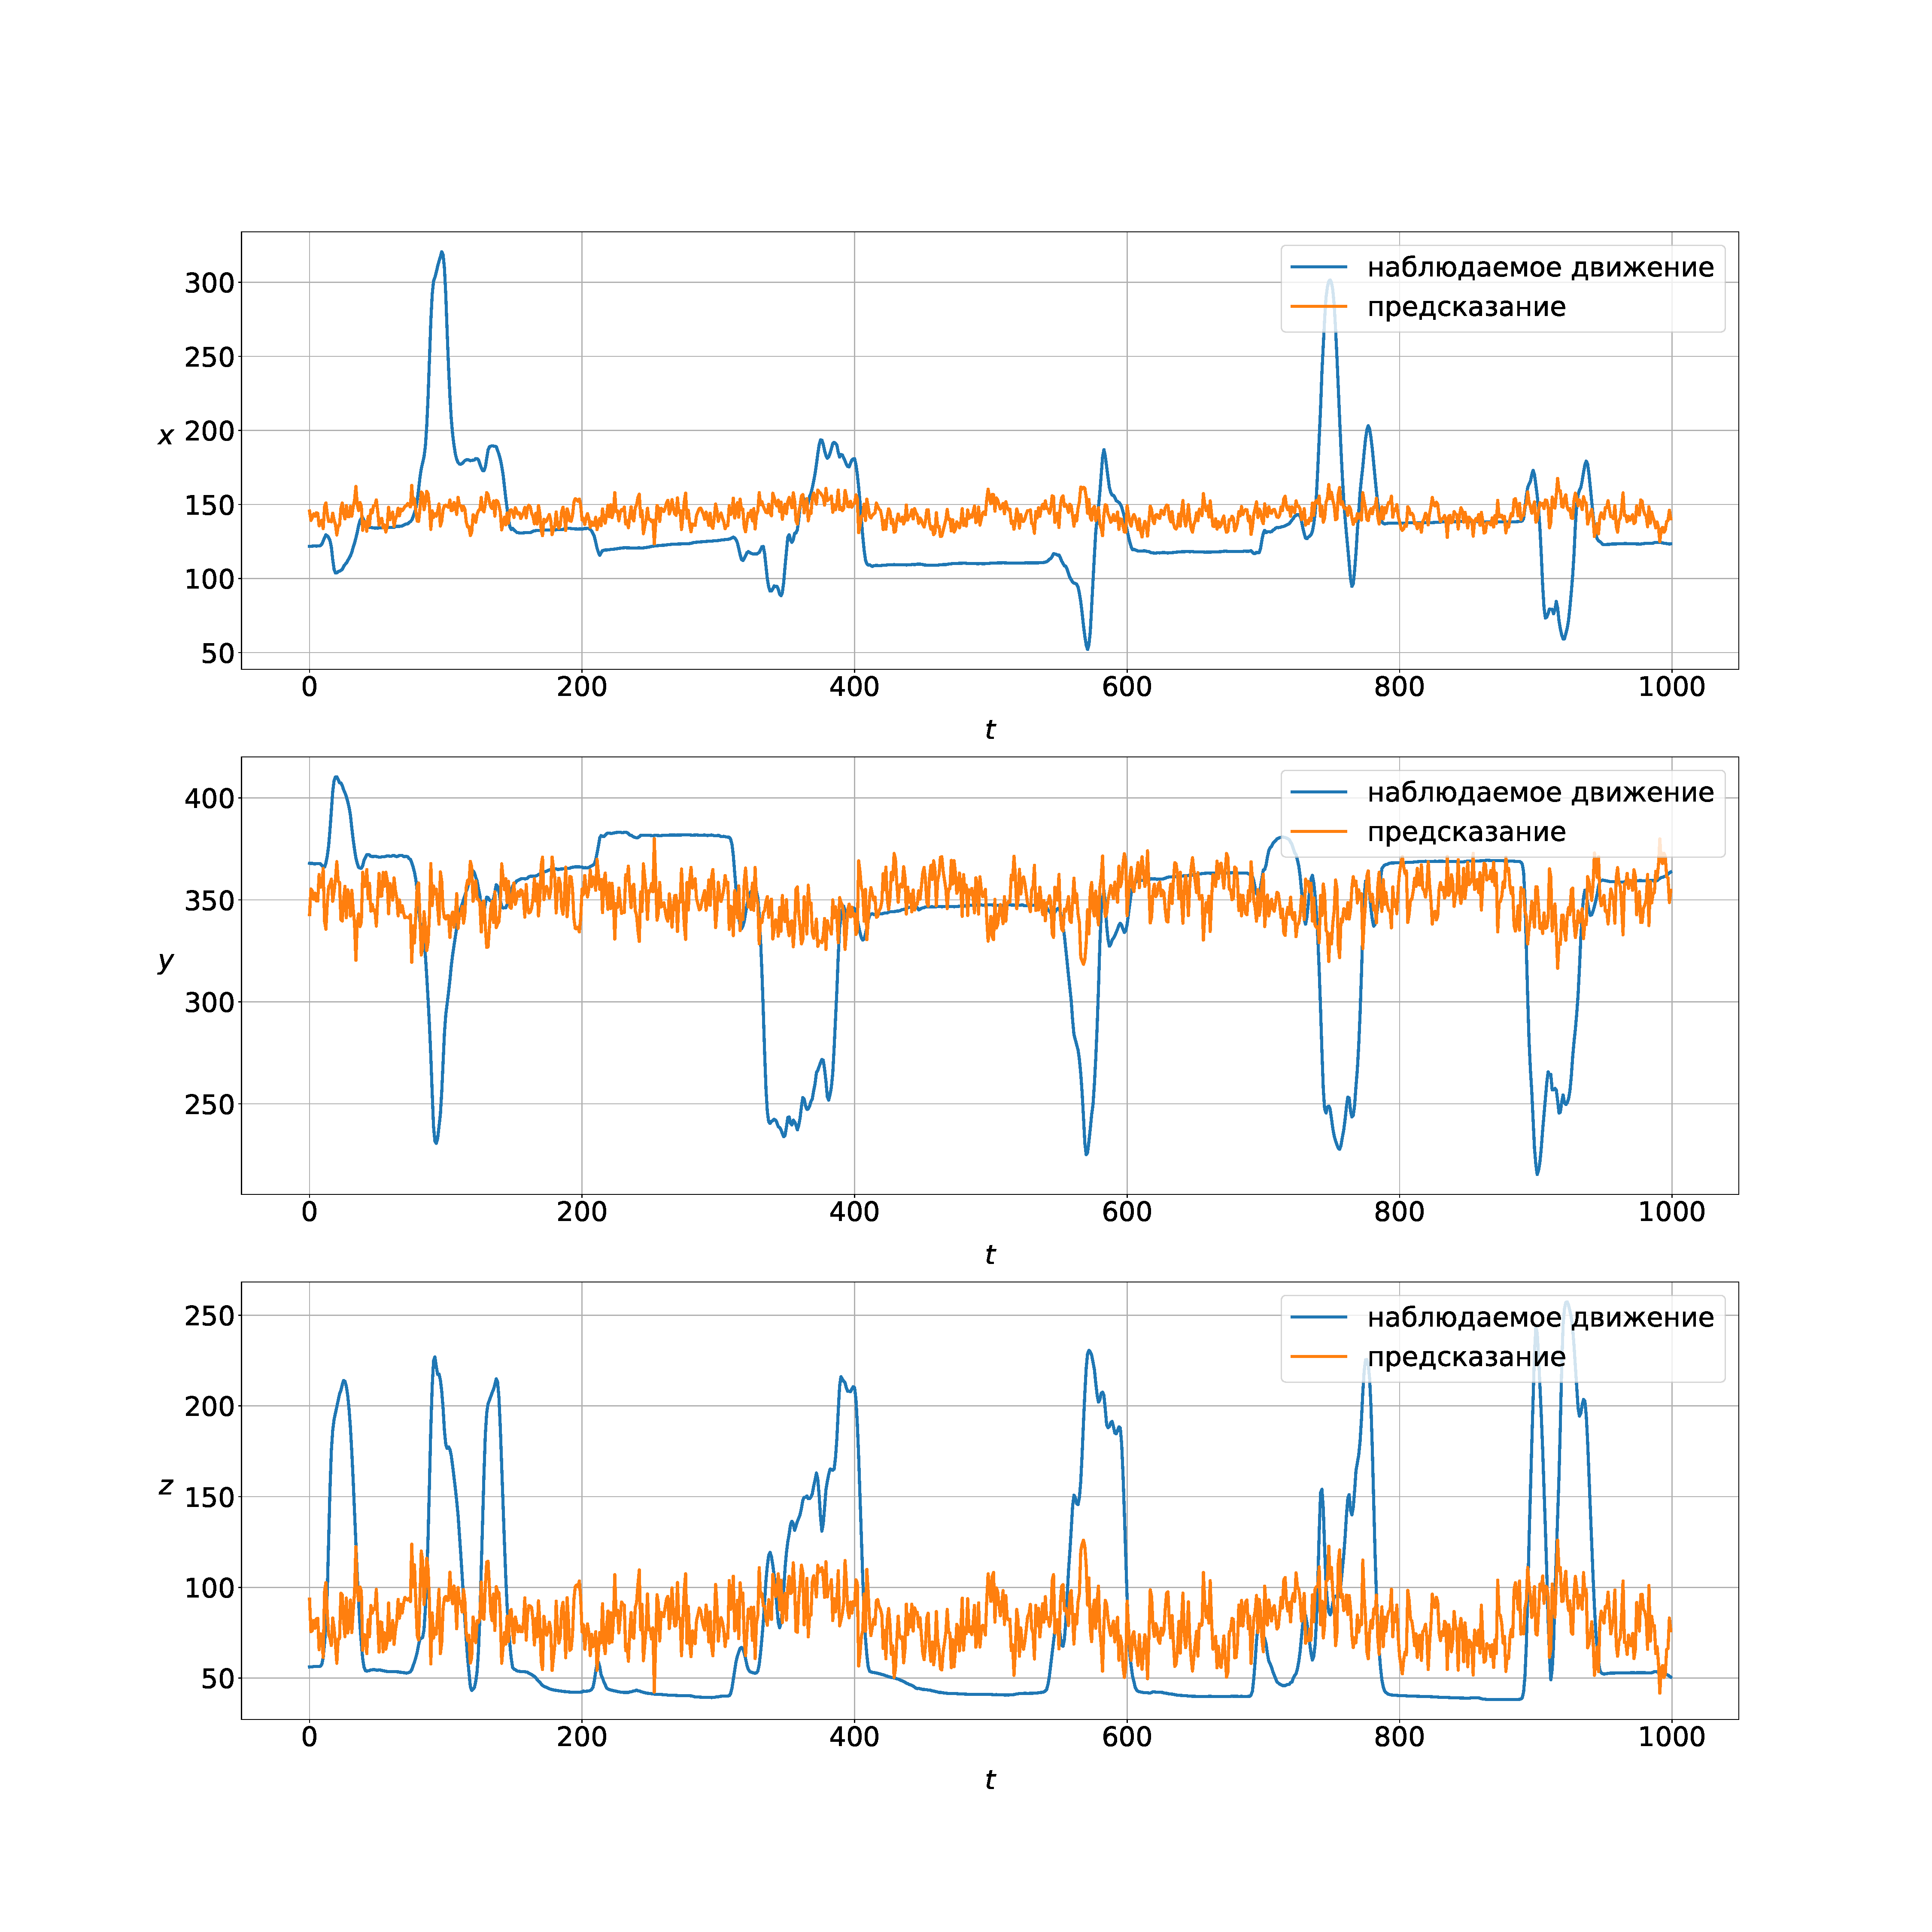
\includegraphics[width=\textwidth]{base_algo.pdf}
    \caption{Предсказания двухкомпонентного PLS, обученного на исходных данных}
    \label{fig:baseAlgo}
  \end{center}
\end{figure}
На графике представлена зависимость координаты конечности от времени. Как видно из рисунка, базовый алгоритм довольно плохо справляется с поставленной задачей. Общий профиль пиков соблюдается, однако PLS очень грубо оценивает острые пики. Также предсказание испытывает флуктуации, когда конечность почти не движется. В результате погрешность предсказания высока. Эксперимент показал значения метрик $mae = 30.17, mse = 1843.91, r2 = 0.01$. Для борьбы с погрешностями предлагается снизить размерность входного сигнала.
